\documentclass{article}

\usepackage[preprint]{tmlr}

\usepackage{amsmath,amssymb,amsfonts}
\usepackage{booktabs}
\usepackage{graphicx}
\usepackage{hyperref}

\renewcommand{\arraystretch}{1.3}
\setlength{\abovetopsep}{6pt}

\title{Grassmannian Geodesic Distance Predicts Cross-Cohort Classifier Degradation\\After Controlling for Source Classifier Quality}

\author{\name Elliot Tower \\
      \email elliot@elliottower.ai}

\begin{document}
\maketitle

\begin{abstract}
Classifiers trained on one cohort routinely degrade when applied to another, yet quantifying this risk before training requires a measure of cross-cohort distributional distance. We propose geodesic distance between cohort-specific PCA subspaces on the Grassmannian manifold $\mathrm{Gr}(k, d)$ as such a measure and test it on seven datasets spanning metagenomics, metabolomics, and gene expression. Raw geodesic--gap correlations are null or weak ($\rho \leq 0.34$) because the AUC gap conflates source classifier quality with distribution shift. After partialing out source internal AUC, geodesic distance predicts the residual gap on a colorectal cancer microbiome meta-analysis (9 studies, 824 samples; partial $\rho = +0.61$, clustered bootstrap 95\% CI $[-0.02, +0.80]$, 97\% positive; $\Delta R^2 = +0.23$) and on the QMDiab multi-biofluid metabolomics study (3 biofluids $\times$ 3 ethnicities, 356 participants; partial $\rho = +0.40$, clustered CI $[+0.04, +0.73]$). Leave-one-study-out prospective validation on the CRC data confirms out-of-sample utility: the geodesic-augmented model reduces prediction MAE by 42\% over baseline and 22\% over a source-quality-only model (mean LOO $\rho = 0.80$). Five additional datasets yield null results, revealing interpretable boundary conditions: the method requires distributional shift driven by analytical heterogeneity (different platforms, protocols, or biological matrices). Centralized platforms (SPIROMICS COPD, TCGA breast cancer) eliminate the variation the geodesic measures, while same-platform gene expression studies (7 independent breast cancer cohorts on Affymetrix HG-U133A, partial $\rho = -0.004$) show that independent study sites alone are insufficient without protocol-level divergence.
\end{abstract}

\section{Introduction}

Clinical metabolomics and microbiome studies routinely report high internal classification accuracy, then fail to reproduce when applied to independent cohorts acquired on different instruments, in different laboratories, or at different times \citep{broadhurst2006statistical}. The transportability gap---the difference between internal cross-validation AUC and external validation AUC---reflects systematic differences in the data-generating process across cohorts: instrument drift, batch effects, population differences, and sample handling variation \citep{wehrens2016improved}.

Domain adaptation theory formalizes this problem. \citet{bendavid2010theory} prove that a classifier's target-domain error is bounded by its source-domain error plus a divergence term between the two distributions. The $\mathcal{H}$-divergence they propose depends on the hypothesis class and requires labeled target data to estimate. A geometry-only surrogate---computable from unlabeled features---would enable prospective flagging of transportability risk before any classifier is trained. Standard batch correction algorithms \citep{johnson2007adjusting} address the problem post hoc; they do not quantify how much the cohort-specific data manifolds diverge.

We propose geodesic distance on the Grassmannian manifold as such a surrogate. Given $C$ cohorts with a shared feature space, we extract the top-$k$ PCA subspace from each, representing each cohort as a point on the Grassmannian $\mathrm{Gr}(k, d)$ \citep{edelman1998geometry}. The geodesic distance between two $k$-dimensional subspaces is the $\ell_2$ norm of their principal angles \citep{bjorck1973numerical, ye2016schubert}:
\begin{equation}
d_{\mathrm{Gr}}(V_1, V_2) = \left(\sum_{i=1}^{k} \theta_i^2\right)^{1/2}
\end{equation}
where $\theta_1, \ldots, \theta_k$ are the principal angles between $V_1$ and $V_2$, obtained as $\theta_i = \arccos(\sigma_i)$ for $\sigma_i$ the singular values of $U_1^\top U_2$ (orthonormal bases $U_1, U_2$). Principal angles of zero indicate shared directions; $\pi/2$ indicates orthogonal directions.

We test this idea on seven datasets spanning different domains: a colorectal cancer (CRC) microbiome meta-analysis (9 independent studies across 7 countries; \citealp{wirbel2019meta}), a multi-biofluid metabolomics study (QMDiab, 3 biofluids $\times$ 3 ethnicities; \citealp{yousri2015metabolic}), a single-study metabolomics dataset (MTBLS7260, 15 analytical plates; \citealp{leonletelier2024contributions}), an inflammatory bowel disease (IBD) metagenomics meta-analysis (5 studies, 1{,}176 samples), a COPD multi-site metabolomics study (SPIROMICS, 8 clinical sites, 584 samples; \citealp{bowler2017spiromics}), a breast cancer gene expression meta-analysis (7 independent Affymetrix HG-U133A studies, 1{,}835 samples), and a TCGA breast cancer RNA-seq analysis (14 tissue source sites, 914 samples).

The AUC gap has a confound that previous work has not addressed: it depends on both the distributional distance between cohorts \emph{and} the quality of the source classifier. A source study with high internal AUC has more room to degrade; one with low internal AUC may transfer well simply because there is little performance to lose. Failing to separate these two components produces null correlations even when the geometric signal is strong.

\paragraph{Contributions.}
\begin{itemize}
\item \textbf{Confound identification (\S\ref{sec:crc}).} The AUC gap conflates source classifier quality ($\rho = +0.68$ with internal AUC) and distribution shift. Raw geodesic--gap correlations are null or weak on all seven datasets.
\item \textbf{Partial correlation (\S\ref{sec:crc}, \S\ref{sec:qmdiab}).} After controlling for source internal AUC, geodesic distance predicts the residual gap on the CRC microbiome data (partial $\rho = +0.61$, clustered bootstrap 95\% CI $[-0.02, +0.80]$, 97\% positive; $\Delta R^2 = +0.23$) and on QMDiab (partial $\rho = +0.40$, clustered CI $[+0.04, +0.73]$). Both results are stable across $k = 5$--$50$ and replicate under alternative distance metrics (chordal) and classifiers (random forest).
\item \textbf{Prospective validation (\S\ref{sec:loo}).} Leave-one-study-out prediction on the CRC data: the geodesic-augmented model achieves mean MAE of 0.057, a 42\% improvement over baseline and 22\% over the source-quality-only model (LOO $\rho = 0.80$).
\item \textbf{Boundary conditions (\S\ref{sec:boundary}).} Five datasets yield null results: IBD metagenomics (5 studies, partial $\rho = -0.11$), COPD multi-site metabolomics (8 sites, partial $\rho = +0.08$), TCGA breast cancer (14 sites, partial $\rho = -0.12$), breast cancer gene expression (7 studies, partial $\rho = -0.004$), and MTBLS7260 metabolomics. The method requires analytical heterogeneity between cohorts; centralized platforms and shared microarray platforms produce null results even across independent study sites.
\item \textbf{Geometric batch detection (\S\ref{sec:batch}).} Cohort subspaces are well-separated from permutation nulls ($z > 25$ on all datasets).
\end{itemize}


\section{Data}

We evaluate on seven datasets spanning different domains and cohort structures (Table~\ref{tab:cohorts}).

\subsection{CRC microbiome meta-analysis (primary)}
\label{sec:crc_data}

The primary dataset comes from the colorectal cancer (CRC) microbiome meta-analysis of \citet{wirbel2019meta} (see also \citealp{thomas2019metaanalysis}), which aggregated shotgun metagenomic data from 9 independent studies across 7 countries (Austria, China, France, Germany, Italy, Japan, United States). We downloaded species-level abundance profiles and sample metadata from Zenodo (record 3517209). After restricting to CRC and healthy control samples, the dataset contains 824 samples across 9 studies, with per-study sizes ranging from 60 to 128. Species with prevalence below 10\% across all samples were removed, yielding 609 features. Abundances were converted to relative proportions and transformed as $\log(1 + 10^6 \cdot p)$ where $p$ is the relative abundance. The 9 studies yield $9 \times 8 = 72$ ordered pairs for the prediction test.

Each study was conducted independently with its own sample collection, DNA extraction, and sequencing protocol, producing genuine cross-laboratory variation. Per-study sample sizes (60--128) and class balance (30--58\% CRC) provide substantially more statistical power for AUC estimation than the metabolomics plates.

\subsection{QMDiab multi-biofluid metabolomics (secondary)}
\label{sec:qmdiab_data}

The QMDiab study \citep{yousri2015metabolic} profiled 356 participants (179 type-2 diabetes, 177 controls) from Qatar on three biofluids: plasma (501 metabolites), urine (734 metabolites), and saliva (289 metabolites). Participants span three ethnic groups: Arab ($n = 200$), Filipino ($n = 108$), and Indian ($n = 34$). We used the preprocessed log$_{10}$-transformed data from Figshare (article 5904022) and restricted to the 89 metabolites measured on all three biofluids. Cohorts are defined by the cross of biofluid and ethnicity (9 cohorts, 72 ordered pairs), producing variation from both biological matrix differences and population structure.

An important distinction from the CRC data: cross-biofluid pairs compare fundamentally different biological matrices (plasma versus urine versus saliva), where the same named metabolite may have different concentration ranges, regulatory mechanisms, and diagnostic relevance. This goes beyond batch effects or instrument calibration---it tests whether subspace geometry tracks biologically meaningful distributional shifts, including cases where the target distribution reflects genuinely different biology.

Cross-biofluid shift produces substantially larger AUC gaps than cross-ethnicity shift: mean gap 0.17 for same-ethnicity cross-biofluid pairs versus 0.02 for same-biofluid cross-ethnicity pairs. Geodesic distances mirror this asymmetry (3.5 cross-biofluid vs 2.5 within-biofluid).

\subsection{MTBLS7260 metabolomics (tertiary)}
\label{sec:metab_data}

MetaboLights accession \textbf{MTBLS7260} \citep{leonletelier2024contributions} is a pancreatic cancer study from the PLCO screening trial containing 1{,}039 serum samples analyzed by LC-MS HILIC for biogenic amines, distributed across 15 analytical plates (PL079--PL093). Each plate contains approximately 72 samples with matched case-control ratio ($\sim$12 cancer, $\sim$60 healthy per plate). After feature alignment, deduplication, and $\log_2$ transformation, the shared feature matrix has 1{,}022 metabolite features per sample. The 15 plates yield $\binom{15}{2} = 105$ unordered pairs (210 ordered) for the prediction test.

Each plate was processed as an independent analytical batch, introducing systematic variation. The critical limitation is statistical power: with $\sim$12 positives per plate, AUC estimates have standard errors of $\sim$0.10, comparable to the total range of observed AUC gaps.

\subsection{IBD metagenomics meta-analysis}
\label{sec:ibd_data}

To test cross-disease generalization, we assembled an IBD metagenomics dataset from the SIAMCAT Zenodo archive \citep{wirbel2021siamcat}. Five studies with IBD (Crohn's disease or ulcerative colitis) and control samples were included: Franzosa 2019 (220 samples), He 2017 (102), HMP2 (106 after subsampling to one timepoint per individual from 1{,}317 longitudinal samples), Lewis 2015 (366), and metaHIT (382). Species-level mOTU v2.5 profiles were merged across studies, yielding 1{,}377 species and 1{,}176 independent samples (781 IBD, 395 control). After prevalence filtering, 547 features remained. The 5 studies yield 20 ordered pairs.

Two studies (HMP2 and Lewis 2015) have severe class imbalance ($\leq$26 controls), and IBD microbiome composition varies substantially with disease activity state (remission versus flare), introducing within-study variance that may exceed between-study distributional shift.

\subsection{SPIROMICS COPD multi-site metabolomics}
\label{sec:copd_data}

To test the method on multi-site metabolomics data with a centralized analytical platform, we used the SPIROMICS COPD study (Metabolomics Workbench ST002088; \citealp{bowler2017spiromics}). Plasma samples from 584 participants (215 current smokers, 369 former smokers) across 8 clinical sites (Columbia, Johns Hopkins, UCLA, UCSF, U of Michigan, U of Utah, Wake Forest University, and Other) were profiled by Metabolon LC-MS. Four analytical modes (two positive, two negative) yielded 1{,}174 metabolites; after filtering to $\geq$50\% prevalence, 909 metabolites remained. All samples were processed on the same centralized Metabolon platform, in contrast to the CRC and IBD datasets where each study used its own laboratory pipeline. The 8 sites yield 56 ordered pairs.

\subsection{Breast cancer gene expression meta-analysis}
\label{sec:brca_geo_data}

To test whether the geodesic method generalizes to gene expression data, we assembled a breast cancer meta-analysis from seven Affymetrix HG-U133A (GPL96) studies deposited in GEO: Wang 2005 (Rotterdam, 286 samples), Desmedt 2007 (Brussels, 198), Pawitan 2005 (Stockholm, 159), Schmidt 2008 (Mainz, 200), Ivshina 2006 (Singapore, 245), Loi 2007 (London, 245), and Hatzis 2011 (Houston, 502). The classification task is estrogen receptor positive (ER+) versus ER-negative, determined from clinical metadata when available (4 studies) or inferred from ESR1 probe expression using a 2-component Gaussian mixture model (3 studies; GMM separation $\geq 2.17$). When ESR1 GMM was used for labeling, ESR1 probes were removed from the feature set. After restricting to probes common across all studies and selecting the 5{,}000 most variable, the merged dataset contains 1{,}835 samples (1{,}263 ER+, 572 ER-) across 7 studies (42 ordered pairs). Expression values were $\log_2$-transformed.

All seven studies used the same Affymetrix HG-U133A platform, which standardizes probe sequences, hybridization chemistry, and signal quantification across laboratories. This shared platform provides a controlled test: studies are independent (different patient populations, sample handling, and RNA extraction protocols) but measure the same features with the same technology.

\subsection{TCGA breast cancer RNA-seq}
\label{sec:tcga_data}

To test the centralized-processing boundary condition on RNA-seq data, we analyzed the TCGA breast cancer cohort (TCGA-BRCA). Gene expression data (RSEM normalized, $\log_2(x+1)$ transformed) were obtained from UCSC Xena; clinical ER status by immunohistochemistry was obtained from cBioPortal. We defined cohorts by tissue source site (TSS), extracted from TCGA barcodes, and restricted to sites with $\geq$25 samples with both expression data and ER status. The resulting dataset contains 914 samples across 14 tissue source sites from institutions including MD Anderson, Pittsburgh, Christiana, and others (182 ordered pairs), using the top 5{,}000 most variable genes. All samples were sequenced centrally by the TCGA consortium using standardized RNA-seq protocols.

\begin{table}[t]
\centering
\caption{Dataset summary. Cohorts are independent studies (CRC, IBD, breast cancer GEO), biofluid--ethnicity groups (QMDiab), analytical plates (MTBLS7260), clinical sites (SPIROMICS), or tissue source sites (TCGA).}
\label{tab:cohorts}
\begin{tabular}{lccccc}
\toprule
Dataset & Cohorts & $n$ per cohort & Features & \% positive & Ordered pairs \\
\midrule
CRC microbiome & 9 studies & 60--128 & 609 & 30--58\% & 72 \\
QMDiab & 9 (3 biofluids $\times$ 3) & 34--200 & 89 & $\sim$50\% & 72 \\
MTBLS7260 & 15 plates & $\sim$72 & 1{,}022 & $\sim$17\% & 210 \\
IBD metagenomics & 5 studies & 102--382 & 547 & 53--93\% & 20 \\
SPIROMICS COPD & 8 sites & 52--117 & 909 & 20--57\% & 56 \\
Breast cancer GEO & 7 studies & 159--502 & 5{,}000 & 56--86\% & 42 \\
TCGA-BRCA & 14 sites & 25--131 & 5{,}000 & 55--85\% & 182 \\
\bottomrule
\end{tabular}
\end{table}


\section{Methods}
\label{sec:methods}

\subsection{Geometric measures}

For each cohort $c$, we compute the top-$k$ PCA subspace $V_c \in \mathrm{Gr}(k, d)$ from its feature matrix. The default subspace dimension is $k = 10$, chosen to capture the dominant variance directions while remaining well below the smallest cohort sample size ($n = 34$ in QMDiab), ensuring stable PCA estimates. We report $k$-sensitivity analyses confirming robustness across $k = 5$--$50$. The geodesic distance between two subspaces is defined in Eq.~1. As a robustness check, we also compute chordal distance $d_{\mathrm{ch}}(V_1, V_2) = \|U_1 U_1^\top - U_2 U_2^\top\|_F$ \citep{conway1996functions}, an alternative metric on $\mathrm{Gr}(k, d)$ that uses projection matrices instead of principal angles. We compute centroid distance ($\|\bar{x}_1 - \bar{x}_2\|_2$) as a baseline that ignores subspace structure.

\subsection{External validation protocol}

For each ordered pair $(i, j)$ of cohorts, we train a logistic regression classifier (L2-regularized, $C = 1$, scikit-learn 1.4) on cohort $i$ using 5-fold stratified cross-validation to estimate internal AUC, then evaluate on cohort $j$ to obtain external AUC. The AUC gap is defined as $\text{AUC}_{\mathrm{int}} - \text{AUC}_{\mathrm{ext}}$; positive values indicate worse external than internal performance. As a robustness check on the CRC data, we repeat the analysis with random forest classifiers (100 trees, max depth 5) to verify that results are not specific to the linear model.

\subsection{Partial correlation}

The AUC gap depends on two quantities: (1) how well the source classifier separates its own data, and (2) how much the target distribution deviates from the source. A source with internal AUC of 0.90 has more headroom to degrade than one at 0.60, so the gap correlates with source quality ($\rho = +0.68$ on the CRC data) independently of any geometric effect. To isolate the geometric contribution, we compute the partial Spearman correlation between geodesic distance and AUC gap, controlling for source internal AUC. We also fit additive OLS models of the form $\mathrm{gap} \sim \mathrm{AUC_{int}} + X$ for each geometric predictor $X$, reporting the $\Delta R^2$ from adding the geometric term.

This decomposition parallels domain adaptation bounds \citep{bendavid2010theory, mansour2009domain}: target error $\leq$ source error $+$ divergence $+$ adaptability. Our partial correlation isolates the divergence component (geodesic distance) after controlling for the source error component (internal AUC).

\subsection{Permutation null}

To test whether cohort subspaces are geometrically distinguishable from chance, we permute cohort labels 200 times: samples are randomly reassigned to cohorts (preserving cohort sizes), PCA subspaces recomputed per group, and mean pairwise geodesic distance recorded. The observed mean is compared to the null distribution by $z$-score.

\subsection{Clustered bootstrap confidence intervals}

Ordered pairs sharing a source or target study are not independent: all pairs with the same source share a classifier and training set. Resampling pairs would underestimate uncertainty by treating these as independent observations. We use a clustered bootstrap that resamples at the study level: each of the $C$ studies is drawn with replacement, and all pairs whose source \emph{and} target both appear in the resampled set are included, with multiplicity proportional to the product of source and target sampling counts. This procedure respects the effective sample size ($C$ studies, not $C(C-1)$ pairs) and produces appropriately wider confidence intervals. We run 2{,}000 iterations and report percentile-based 95\% CIs.

\subsection{$k$-sensitivity}

To assess robustness to subspace dimension, we repeat the partial correlation analysis at $k \in \{5, 10, 15, 20, 30, 50\}$.

All analyses use Python 3.11 with NumPy 1.26, SciPy 1.12, and scikit-learn 1.4.


\section{Results}

\subsection{Geometric batch detection}
\label{sec:batch}

Cohort subspaces are well-separated from permutation nulls on all datasets tested. On MTBLS7260, the observed mean geodesic distance (3.604) falls entirely outside the null distribution (null mean $3.169 \pm 0.016$, $z = 27.47$, $p < 0.001$; Figure~\ref{fig:null_metab}). Distances range from 3.25 to 3.82 with a coefficient of variation of 3.5\%, indicating that all plates are roughly equidistant on the Grassmannian. The angle spectrum confirms that even the closest plate pair shares no near-zero principal angles.

On the CRC microbiome data, the separation is comparable: observed mean geodesic 3.628 versus null mean $3.125 \pm 0.020$, $z = 25.67$, $p < 0.001$ (Figure~\ref{fig:null_crc}). The wider range of geodesic distances across study pairs (2.98--4.12) reflects the greater heterogeneity expected from independent laboratories.

\begin{figure}[t]
\centering
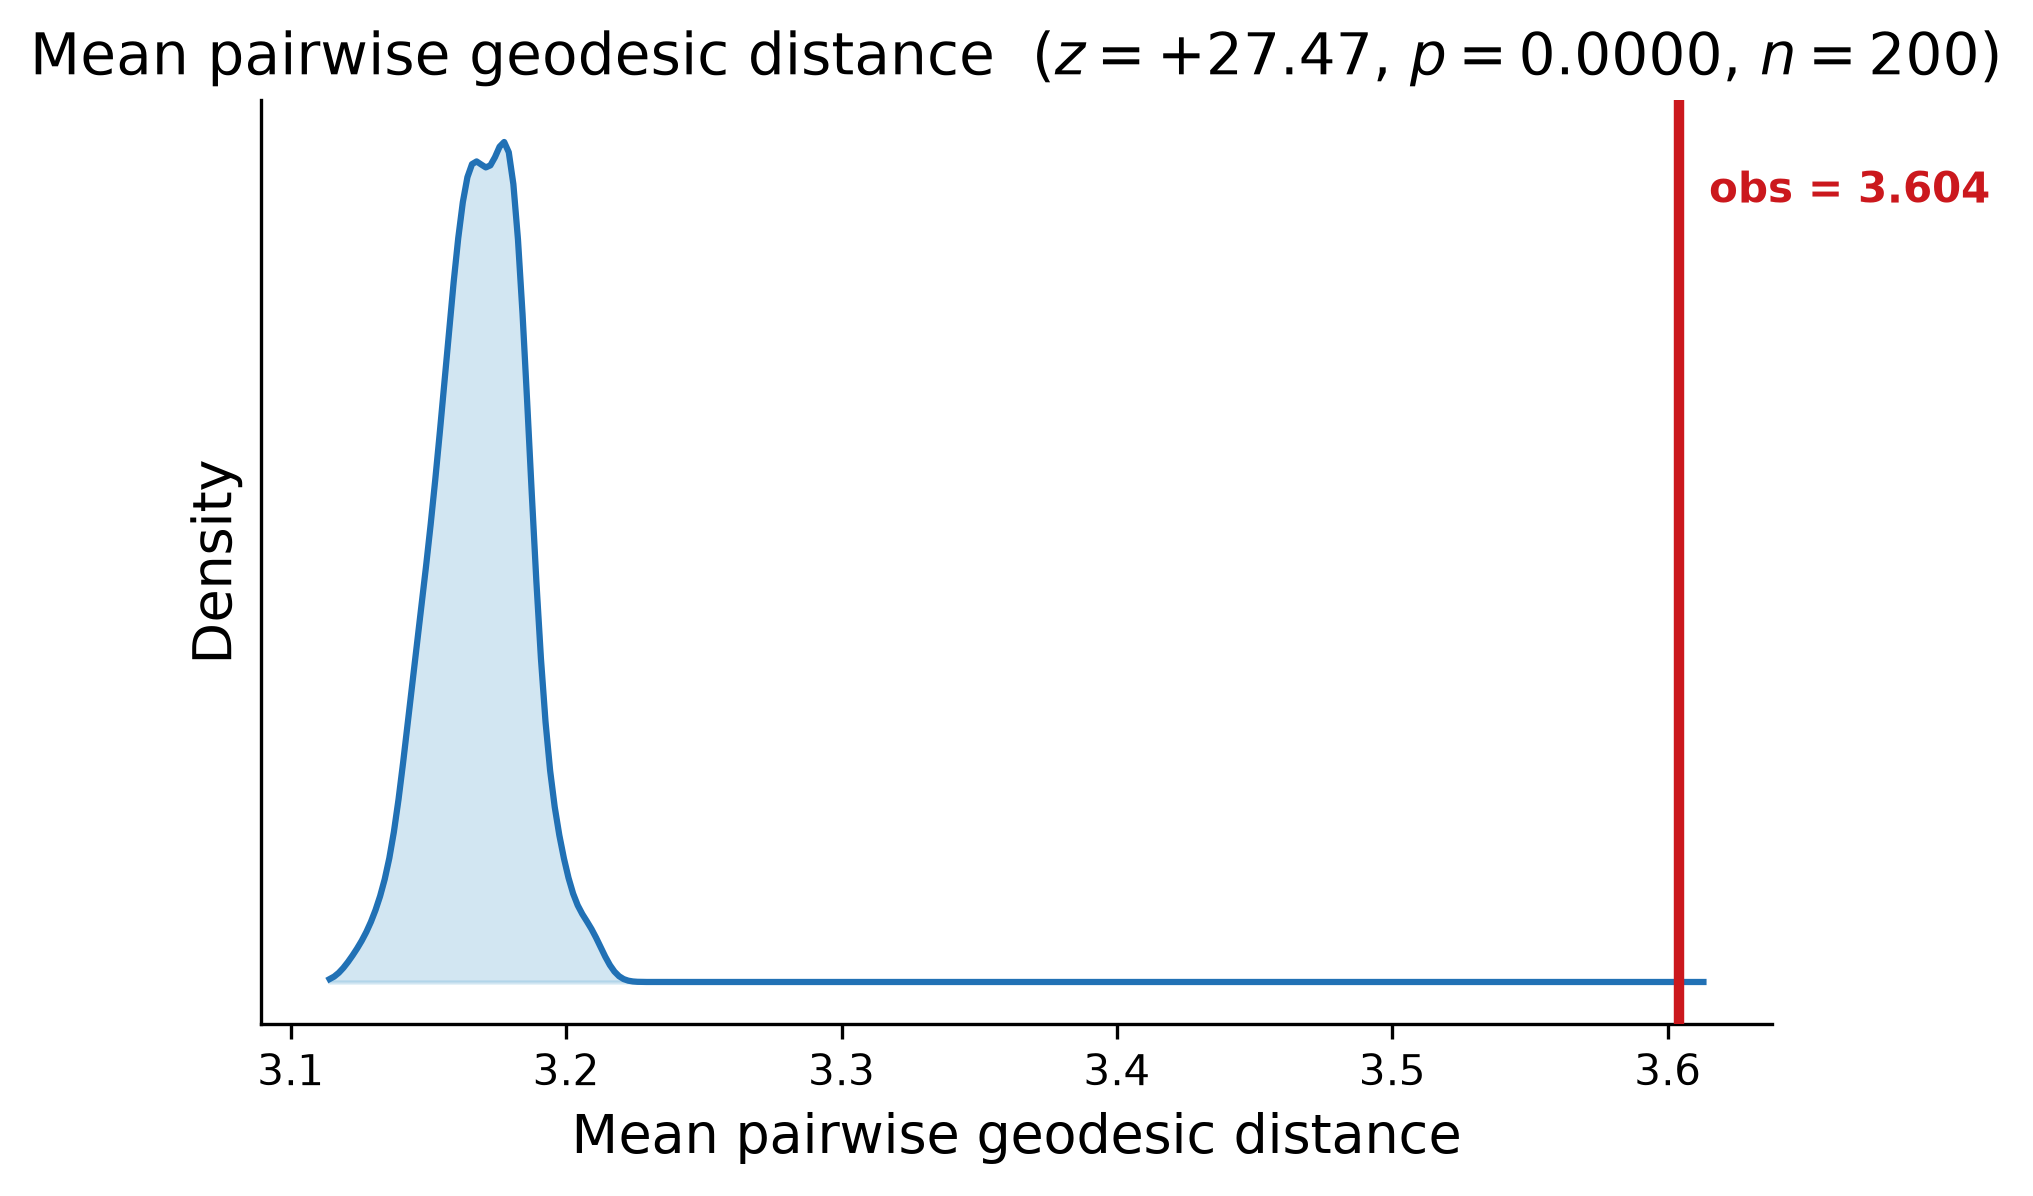
\includegraphics[width=0.7\textwidth]{results/multicohort/figures/F3_null_multicohort.png}
\caption{MTBLS7260: mean pairwise geodesic distance (observed $= 3.604$, red line) against the plate-label permutation null (200 permutations, $z = 27.47$). The observed value falls entirely outside the null support.}
\label{fig:null_metab}
\end{figure}

\begin{figure}[t]
\centering
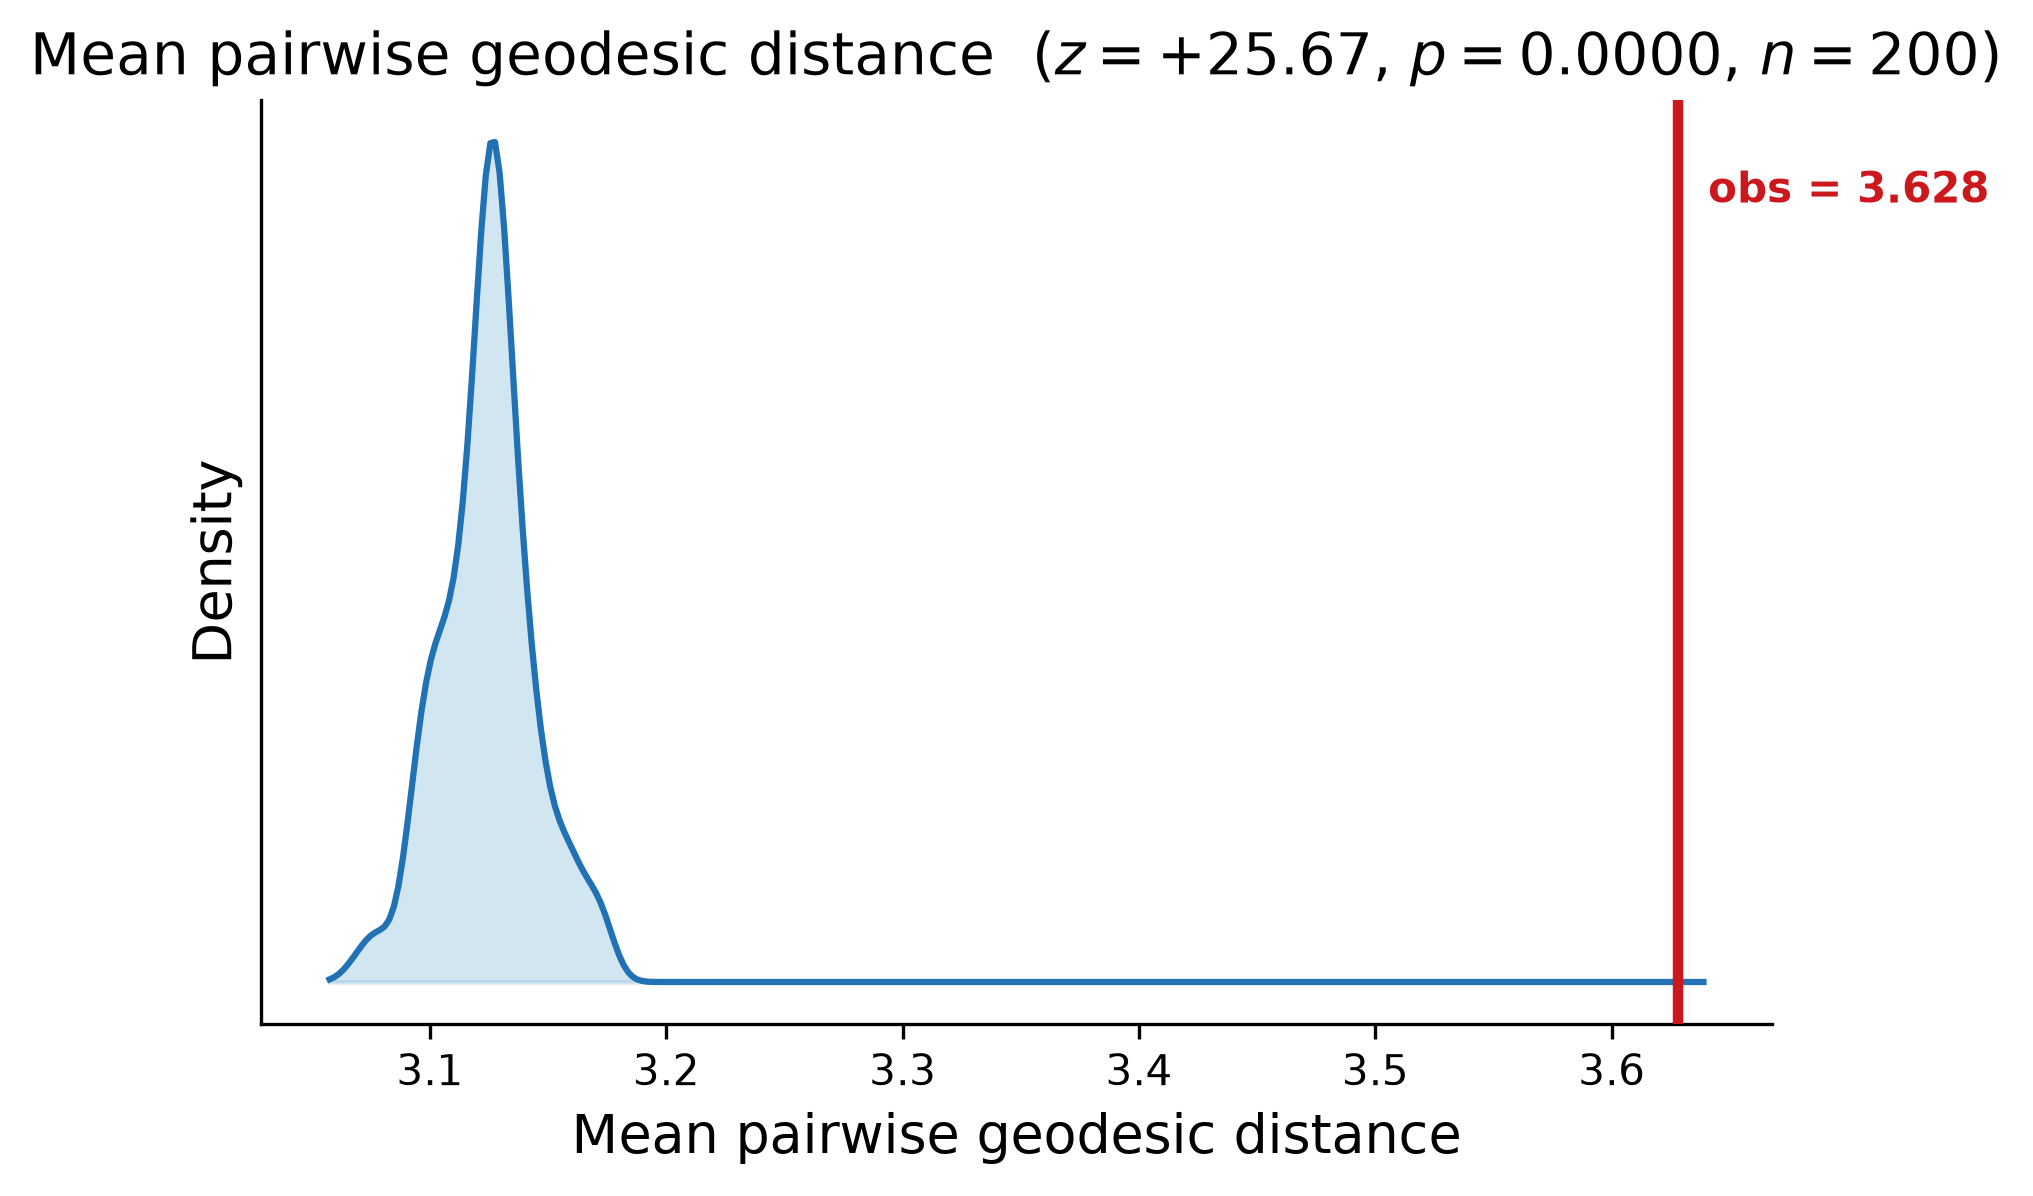
\includegraphics[width=0.7\textwidth]{microbiome-crc/results/figures/F2_null_model.png}
\caption{CRC microbiome: mean pairwise geodesic distance (observed $= 3.628$, red line) against the study-label permutation null (200 permutations, $z = 25.67$). Study subspaces are well-separated from chance.}
\label{fig:null_crc}
\end{figure}


\subsection{CRC microbiome: partial correlation reveals geometric signal}
\label{sec:crc}

Raw Spearman correlations between each geometric predictor and the AUC gap are null across all 72 ordered pairs (Table~\ref{tab:raw_crc}). Geodesic distance achieves $\rho = +0.118$ ($p = 0.32$), centroid distance $\rho = +0.090$ ($p = 0.45$), and two directional predictors---Fisher discriminant projection and bracket-norm decomposition---perform no better.

\begin{table}[t]
\centering
\caption{CRC microbiome: Spearman $\rho$ between each predictor and the AUC gap. Left: raw correlations (all null). Right: partial correlations controlling for source internal AUC. Geodesic distance emerges as a strong predictor after the correction.}
\label{tab:raw_crc}
\begin{tabular}{lcccc}
\toprule
 & \multicolumn{2}{c}{Raw} & \multicolumn{2}{c}{Partial $|$ int.\ AUC} \\
\cmidrule(lr){2-3} \cmidrule(lr){4-5}
Predictor & $\rho$ & $p$ & $\rho$ & $p$ \\
\midrule
Geodesic distance        & $+$0.118 & 0.324 & $+$0.613 & $<$0.0001 \\
Centroid distance        & $+$0.090 & 0.453 & $+$0.396 & 0.0006 \\
Bracket-norm             & $-$0.020 & 0.869 & $-$0.383 & 0.0009 \\
Directional transport    & $+$0.024 & 0.840 & $-$0.106 & 0.375 \\
\bottomrule
\end{tabular}
\end{table}

The reason is a confound. The AUC gap correlates strongly with source internal AUC ($\rho = +0.677$, $p < 0.0001$): studies with better internal classifiers show larger drops on external data. Source quality accounts for 47\% of the variance in the gap ($R^2 = 0.467$ for $\text{gap} \sim \text{AUC}_{\mathrm{int}}$). This correlation masks any geometric signal because studies with high internal AUC also tend to have distinctive subspace geometry.

After partialing out source internal AUC, geodesic distance becomes the strongest predictor of the residual gap (partial $\rho = +0.613$, $p < 0.0001$; Figure~\ref{fig:partial}). In a multivariate OLS model, adding geodesic distance to source AUC improves $R^2$ from 0.467 to 0.693 ($\Delta R^2 = +0.226$). Centroid distance provides a smaller improvement ($\Delta R^2 = +0.081$), and the directional transport predictor adds nothing ($\Delta R^2 = +0.006$; Table~\ref{tab:multivariate}).

Clustered bootstrap resampling---which resamples the 9 studies rather than the 72 pairs (see \S\ref{sec:methods})---confirms the stability of this result. With random forest classifiers, the clustered 95\% CI is $[+0.03, +0.77]$ (median partial $\rho = +0.53$, 98\% positive). With logistic regression, the CI is $[-0.02, +0.80]$ (median $+0.56$, 97\% positive). The wider CIs relative to naive pair-level resampling reflect the effective sample size of 9 studies rather than 72 pairs.

The result is robust to alternative distance metrics and classifiers. Chordal distance---which measures $\|U_1 U_1^\top - U_2 U_2^\top\|_F$ rather than aggregating principal angles---achieves partial $\rho = +0.55$ with clustered CI $[-0.06, +0.79]$. Random forest classifiers yield the same partial $\rho = +0.58$ as logistic regression, confirming that the geometric signal is not specific to linear classifiers.

\begin{table}[t]
\centering
\caption{Multivariate OLS models: $\text{gap} \sim \text{AUC}_{\mathrm{int}} + X$. Adding geodesic distance to the source-quality baseline yields the largest $R^2$ improvement.}
\label{tab:multivariate}
\begin{tabular}{lcc}
\toprule
Model & $R^2$ & $\Delta R^2$ \\
\midrule
AUC$_{\mathrm{int}}$ only & 0.467 & --- \\
$+$ geodesic distance     & 0.693 & $+$0.226 \\
$+$ bracket-norm          & 0.558 & $+$0.091 \\
$+$ centroid distance     & 0.549 & $+$0.081 \\
$+$ directional transport & 0.473 & $+$0.006 \\
\bottomrule
\end{tabular}
\end{table}

\begin{figure}[t]
\centering
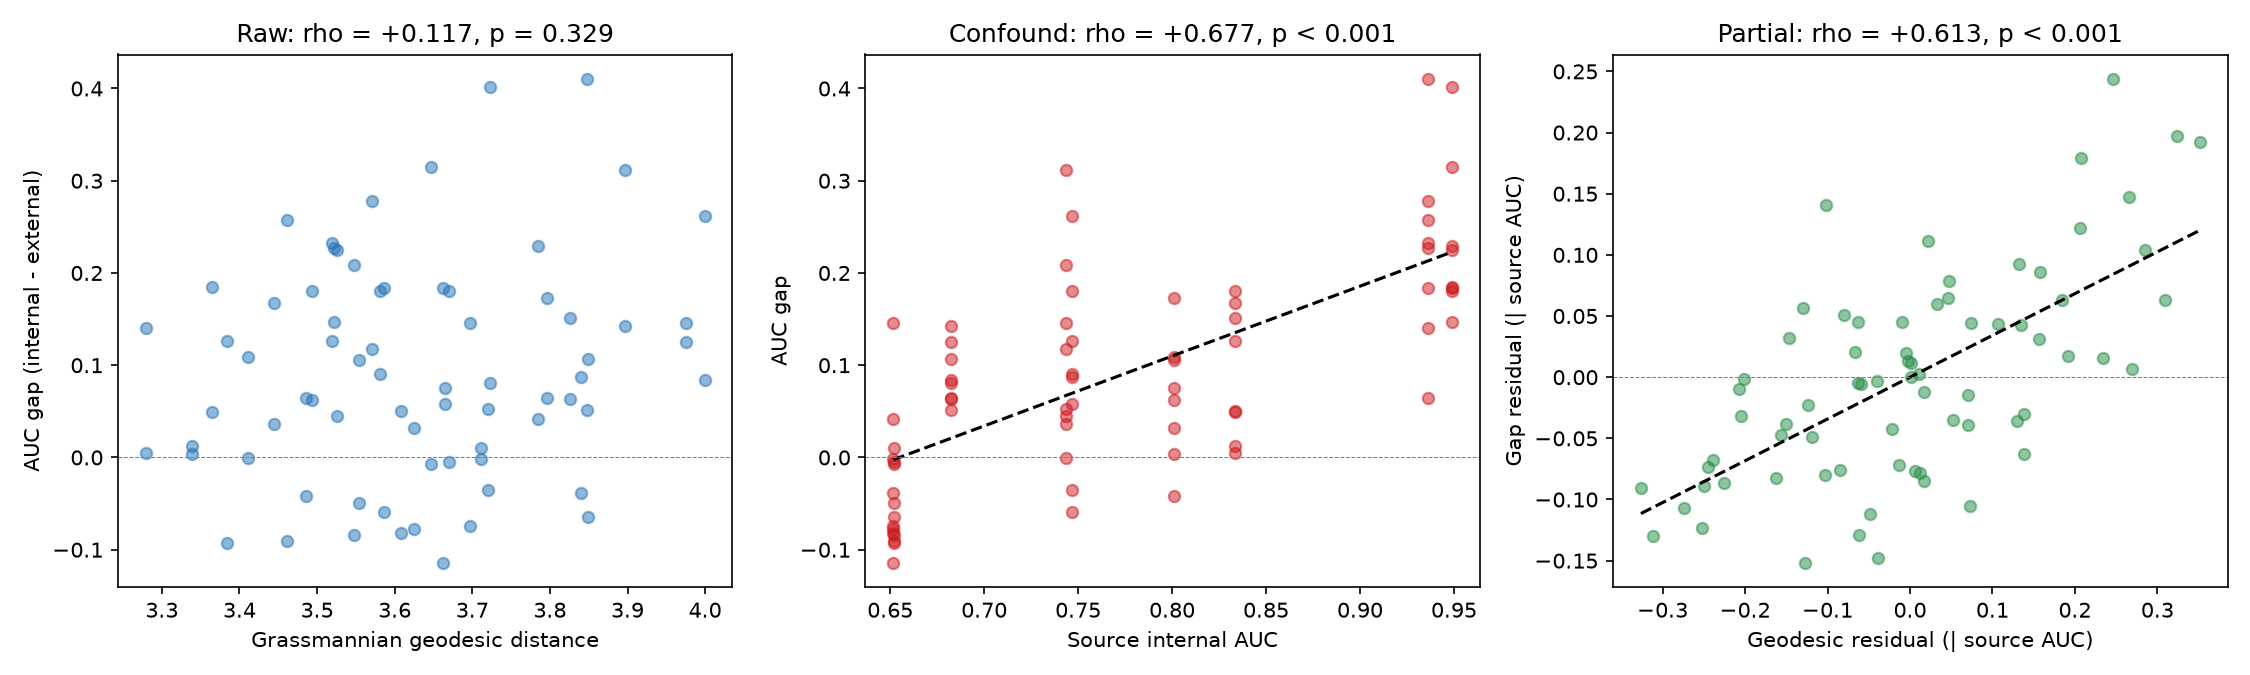
\includegraphics[width=\textwidth]{microbiome-crc/results/figures/F1_partial_correlation.png}
\caption{Three views of the geodesic--gap relationship on the CRC data. Left: raw Spearman correlation is null ($\rho = +0.12$). Center: source internal AUC is the dominant confound ($\rho = +0.68$ with gap). Right: after partialing out source AUC, geodesic distance is strongly predictive (partial $\rho = +0.61$, $p < 0.0001$).}
\label{fig:partial}
\end{figure}

The partial correlation is robust across subspace dimensions (Table~\ref{tab:ksens}). Raw correlations are null at every $k$, while partial correlations stabilize between $+0.56$ and $+0.63$ for $k = 10$ to $k = 50$, peaking at $k = 20$ ($\rho = +0.634$). The result is insensitive to the choice of $k$ across a five-fold range.

\begin{table}[t]
\centering
\caption{$k$-sensitivity: raw and partial Spearman $\rho$ between geodesic distance and AUC gap at different subspace dimensions. Raw correlations are null at all $k$; partial correlations are stable.}
\label{tab:ksens}
\begin{tabular}{lcccc}
\toprule
$k$ & Raw $\rho$ & $p$ (raw) & Partial $\rho$ & $p$ (partial) \\
\midrule
5  & $+$0.100 & 0.405 & $+$0.413 & 0.0003 \\
10 & $+$0.117 & 0.326 & $+$0.613 & $<$0.0001 \\
15 & $+$0.092 & 0.444 & $+$0.627 & $<$0.0001 \\
20 & $+$0.097 & 0.416 & $+$0.634 & $<$0.0001 \\
30 & $+$0.067 & 0.574 & $+$0.571 & $<$0.0001 \\
50 & $+$0.057 & 0.634 & $+$0.557 & $<$0.0001 \\
\bottomrule
\end{tabular}
\end{table}


\subsection{QMDiab: cross-biofluid and cross-ethnicity validation}
\label{sec:qmdiab}

The QMDiab dataset provides cross-biofluid and cross-ethnicity variation in a single study. Across 72 ordered pairs, raw Spearman correlations are already moderate for centroid distance ($\rho = +0.628$, $p < 10^{-8}$) and geodesic distance ($\rho = +0.337$, $p = 0.004$), driven by the large cross-biofluid effect. After partialing out source internal AUC, geodesic distance strengthens to partial $\rho = +0.404$ ($p < 0.001$) and centroid distance to partial $\rho = +0.659$ ($p < 10^{-9}$; Table~\ref{tab:qmdiab}).

Centroid distance dominates geodesic distance on this dataset because the primary variation is cross-biofluid: plasma, urine, and saliva produce large centroid shifts in metabolite concentrations, so a simple Euclidean distance captures most of the signal. The geodesic captures additional subspace-level structure beyond the centroid shift, as shown by its improvement under partial correlation ($+0.337 \to +0.404$), but starts from a lower baseline when centroid shifts are extreme.

A multivariate model ($\text{gap} \sim \text{AUC}_{\mathrm{int}} + \text{geodesic}$) achieves $R^2 = 0.397$, confirming that geodesic distance adds predictive value beyond source quality. As on the CRC data, directional transport contributes nothing in the signed form ($\rho = +0.08$); its absolute value performs moderately ($\rho = +0.47$), suggesting the magnitude of the discriminant projection tracks the cross-biofluid shift even though its sign is uninformative.

\begin{table}[t]
\centering
\caption{QMDiab: raw and partial Spearman $\rho$ between each predictor and the AUC gap (72 ordered pairs, 9 cohorts). Centroid distance dominates due to the large cross-biofluid shift; geodesic distance strengthens after partialing out source AUC.}
\label{tab:qmdiab}
\begin{tabular}{lcccc}
\toprule
 & \multicolumn{2}{c}{Raw} & \multicolumn{2}{c}{Partial $|$ int.\ AUC} \\
\cmidrule(lr){2-3} \cmidrule(lr){4-5}
Predictor & $\rho$ & $p$ & $\rho$ & $p$ \\
\midrule
Centroid distance        & $+$0.628 & $<10^{-8}$ & $+$0.659 & $<10^{-9}$ \\
Dir.\ transport (abs)    & $+$0.487 & $<10^{-4}$ & $+$0.472 & $<10^{-4}$ \\
Geodesic distance        & $+$0.337 & 0.004      & $+$0.404 & $<$0.001 \\
Bracket-norm             & $-$0.411 & $<$0.001   & $-$0.401 & $<$0.001 \\
Dir.\ transport (signed) & $+$0.158 & 0.184      & $+$0.079 & 0.514 \\
\bottomrule
\end{tabular}
\end{table}

The same partial-correlation pattern visible on the CRC data appears here (Figure~\ref{fig:partial_qmdiab}): the raw geodesic--gap scatter shows a weak trend that strengthens after removing the source-quality component.

The partial correlation is robust across subspace dimensions (Table~\ref{tab:ksens_qmdiab}, Figure~\ref{fig:ksens_qmdiab}). Unlike the CRC data where raw correlations are null at every $k$, QMDiab raw correlations are already significant ($\rho = +0.32$ to $+0.42$) due to the strong cross-biofluid effect. Partial correlations stabilize between $+0.40$ and $+0.50$ for $k = 5$ to $k = 50$, peaking at $k = 30$ ($\rho = +0.498$). Clustered bootstrap resampling (resampling the 9 cohorts) confirms: median partial $\rho = +0.38$, 95\% CI $[+0.04, +0.73]$, with 99\% of 2{,}000 samples positive.

\begin{figure}[t]
\centering
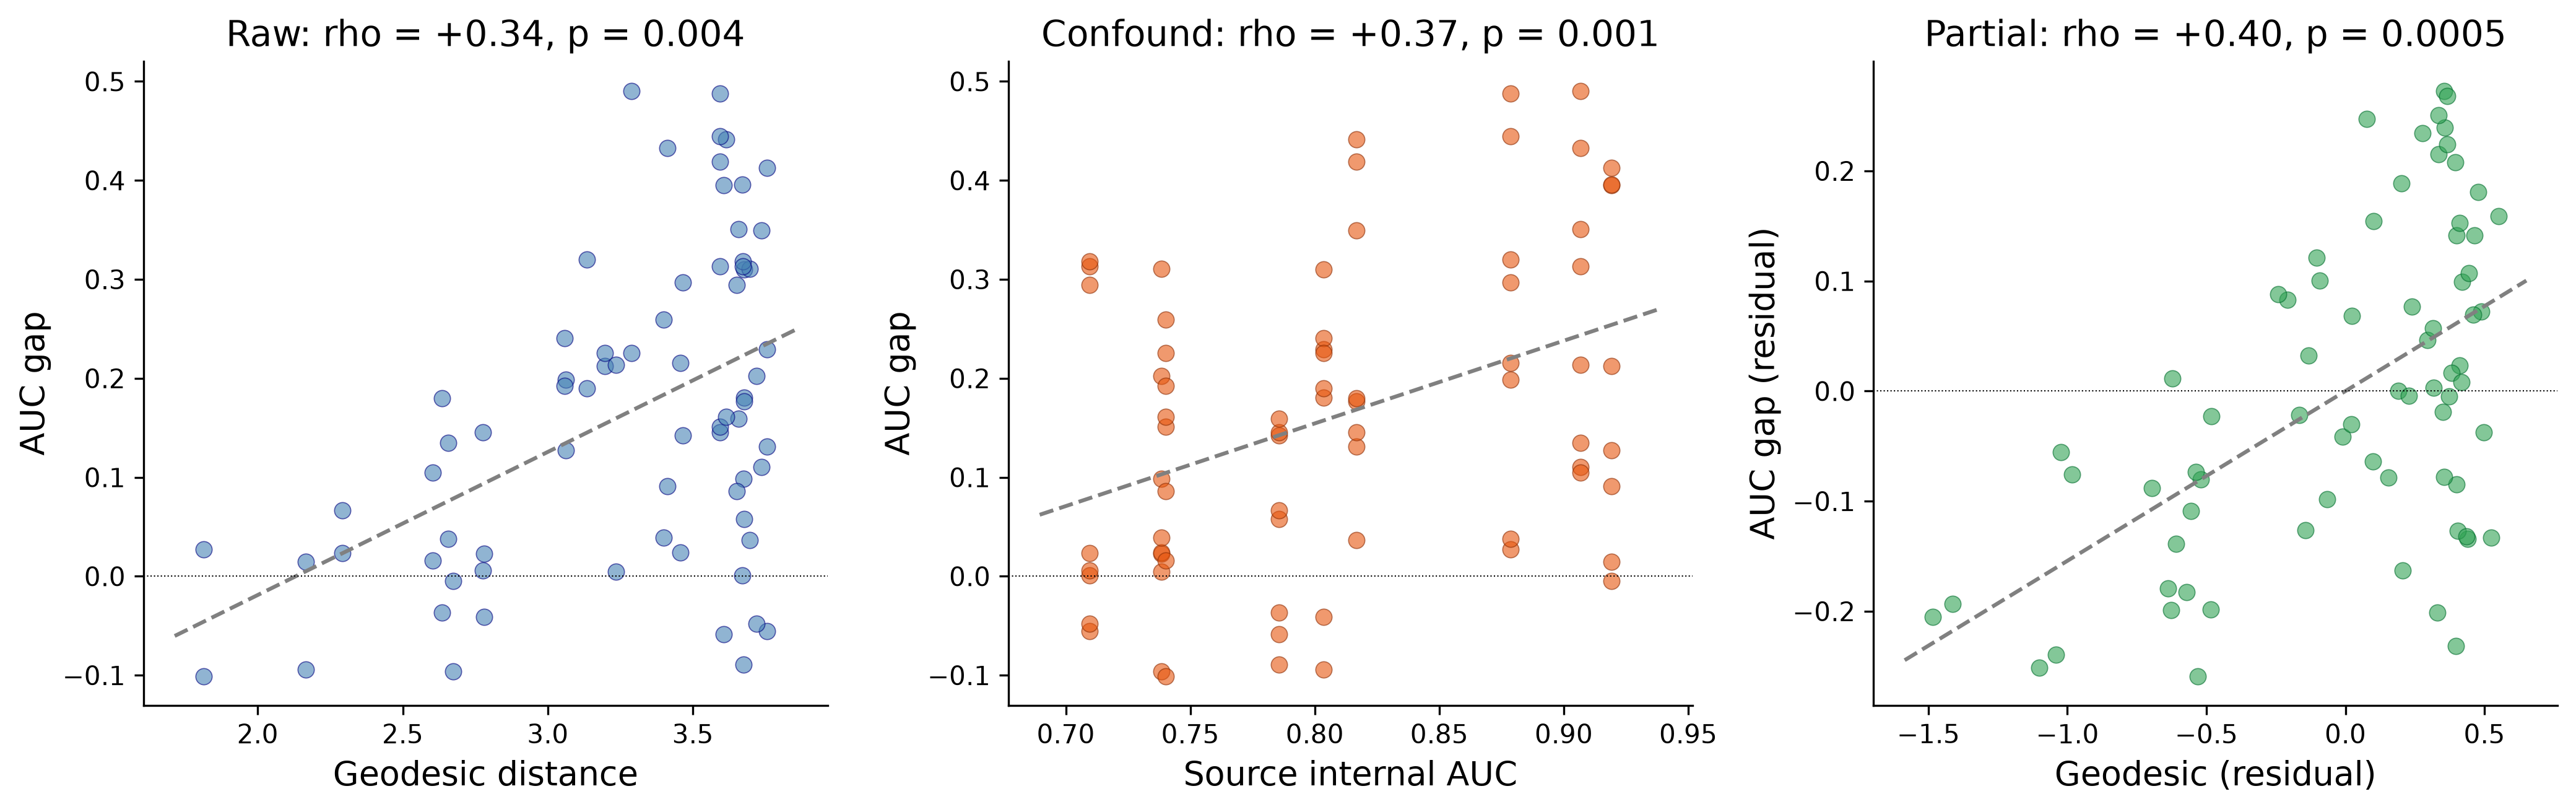
\includegraphics[width=\textwidth]{metabolomics-multilab/results/figures/F1_qmdiab_partial_correlation.png}
\caption{Three views of the geodesic--gap relationship on the QMDiab data. Left: raw correlation is weak ($\rho = +0.34$). Center: source internal AUC correlates with gap. Right: after partialing out source AUC, geodesic distance is predictive (partial $\rho = +0.40$, $p < 0.001$).}
\label{fig:partial_qmdiab}
\end{figure}

\begin{figure}[t]
\centering
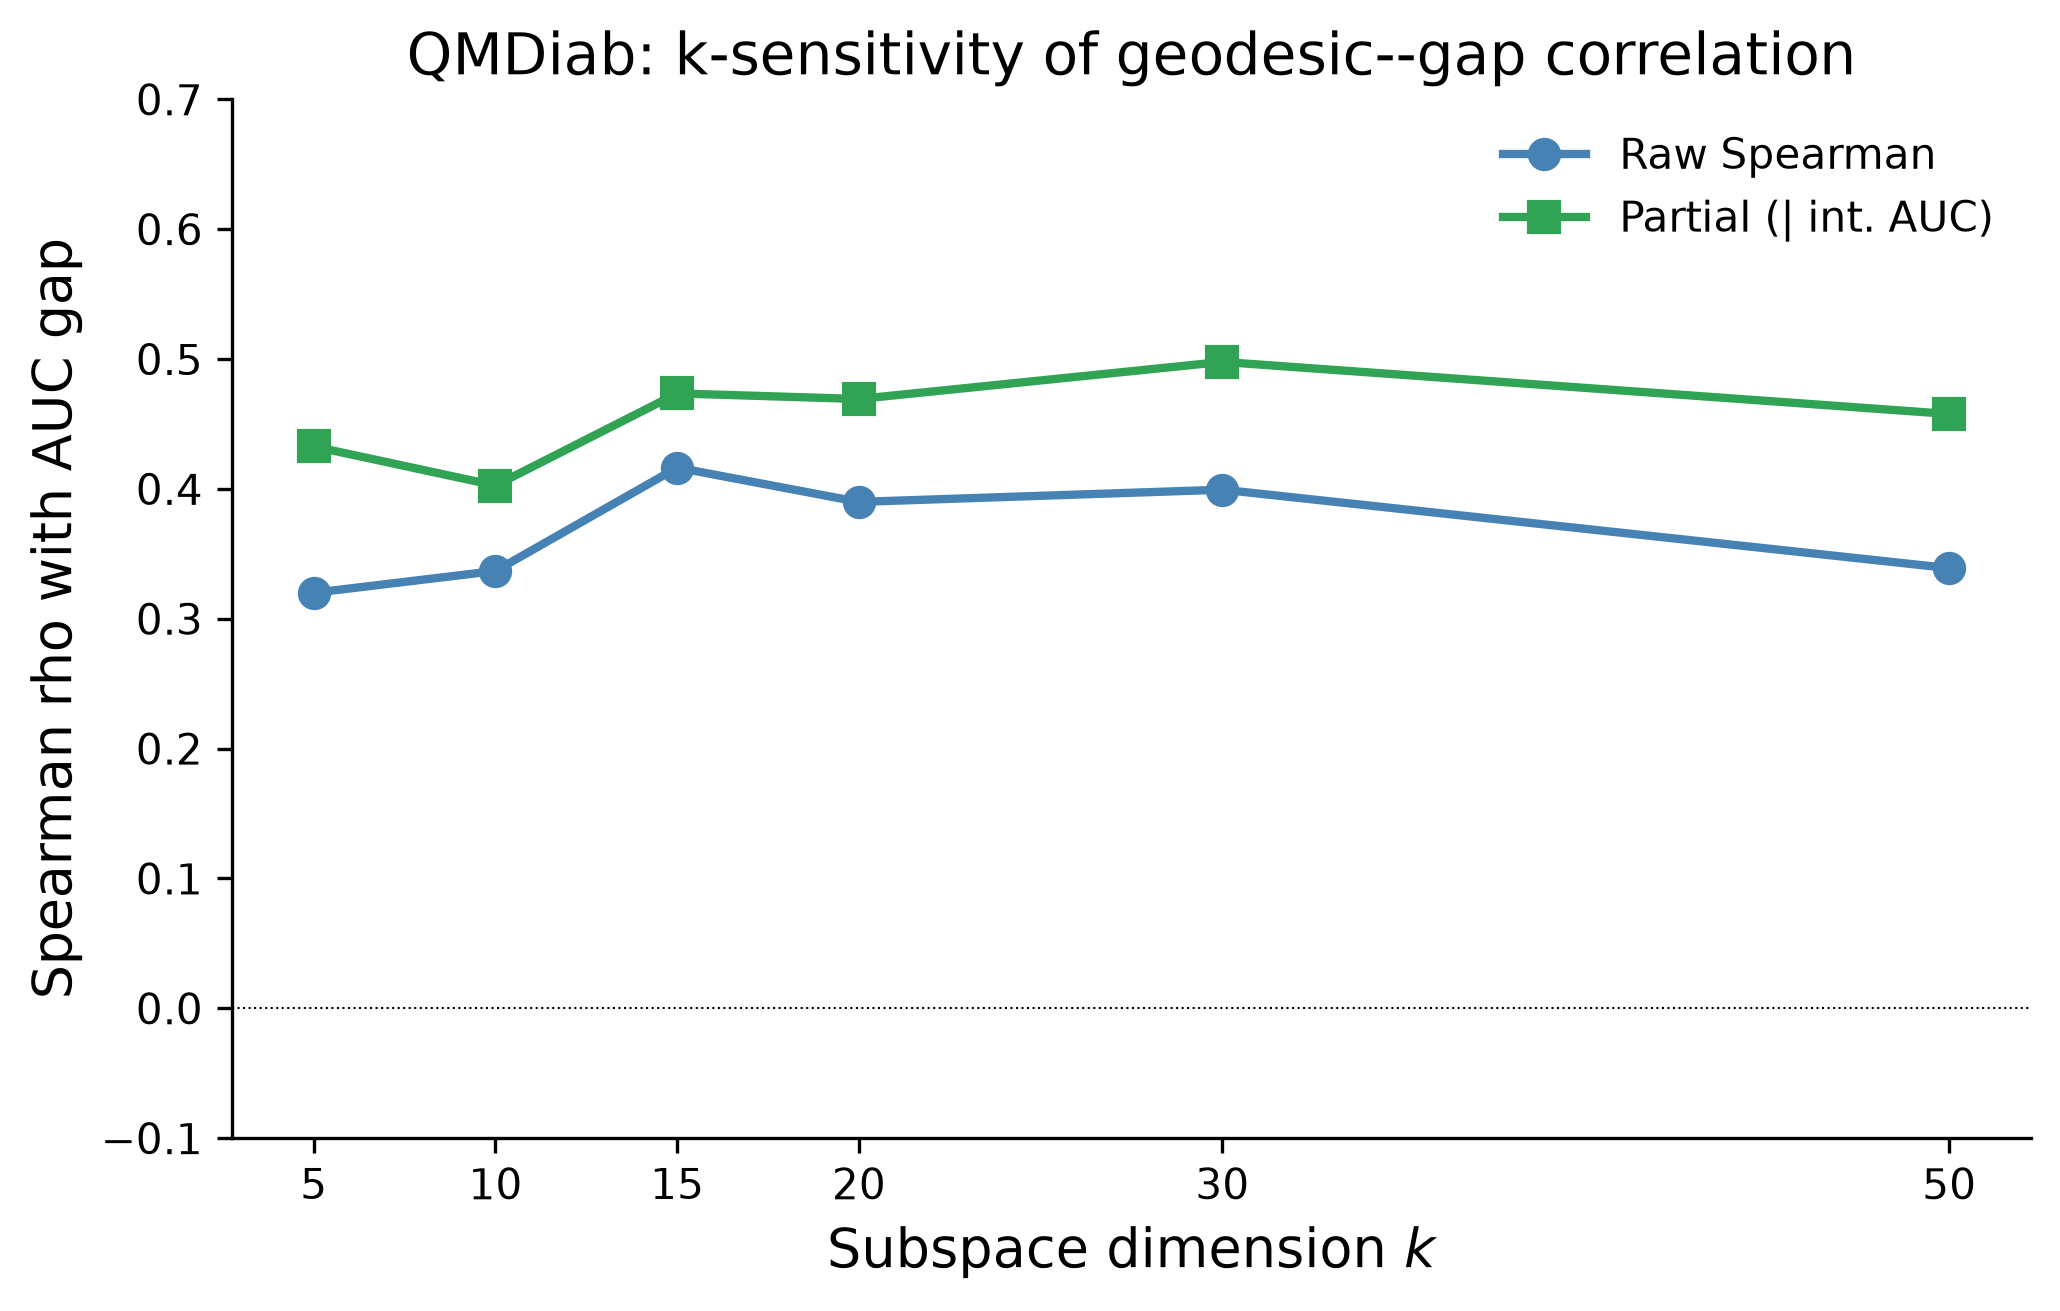
\includegraphics[width=0.7\textwidth]{metabolomics-multilab/results/figures/F2_qmdiab_k_sensitivity.png}
\caption{QMDiab $k$-sensitivity. Raw correlations (blue) are significant at all $k$ due to the strong cross-biofluid effect. Partial correlations (green) are stronger and stable across $k = 5$--$50$.}
\label{fig:ksens_qmdiab}
\end{figure}

\begin{table}[t]
\centering
\caption{QMDiab $k$-sensitivity: raw and partial Spearman $\rho$ between geodesic distance and AUC gap. Both raw and partial correlations are significant and stable across $k$.}
\label{tab:ksens_qmdiab}
\begin{tabular}{lcccc}
\toprule
$k$ & Raw $\rho$ & $p$ (raw) & Partial $\rho$ & $p$ (partial) \\
\midrule
5  & $+$0.320 & 0.006 & $+$0.433 & 0.0002 \\
10 & $+$0.337 & 0.004 & $+$0.403 & 0.0005 \\
15 & $+$0.416 & 0.0003 & $+$0.474 & $<$0.0001 \\
20 & $+$0.390 & 0.0007 & $+$0.469 & $<$0.0001 \\
30 & $+$0.399 & 0.0005 & $+$0.498 & $<$0.0001 \\
50 & $+$0.339 & 0.004 & $+$0.458 & $<$0.0001 \\
\bottomrule
\end{tabular}
\end{table}


\subsection{MTBLS7260 metabolomics: noise floor prevents detection}
\label{sec:metabolomics}

On the metabolomics data, all raw correlations between geometric predictors and the AUC gap are null ($|\rho| \leq 0.19$, all $p > 0.05$; Table~\ref{tab:baselines_metab}). The partial correlation correction applied to the CRC data does not rescue the result: source internal AUC itself is too noisy to serve as a useful covariate. With $\sim$12 positives per plate, the standard error of each internal AUC estimate is $\sim$0.10, comparable to the total range of observed gaps ($-0.44$ to $+0.44$). The confound-correction approach requires that the confound (source quality) be measurable with reasonable precision; when it is not, partialing out a noisy estimate attenuates rather than sharpens the residual signal.

The geodesic distances are also compressed (CV 3.5\%), reflecting the mild batch regime of plates within a single study. Taken together, the metabolomics null is consistent with insufficient statistical power for both the source quality signal and the geometric signal, rather than absence of the underlying relationship.

\begin{table}[t]
\centering
\caption{MTBLS7260: Spearman $\rho$ between each score and the AUC gap (logistic regression classifier, 210 ordered pairs). All correlations are non-significant.}
\label{tab:baselines_metab}
\begin{tabular}{lcc}
\toprule
Score & $\rho$ & $p$ \\
\midrule
Geodesic distance     & $+$0.040 & 0.684 \\
Centroid distance     & $+$0.157 & 0.110 \\
Domain-classifier AUC & $-$0.092 & 0.350 \\
Variance ratio        & $+$0.188 & 0.054 \\
\bottomrule
\end{tabular}
\end{table}


\subsection{Leave-one-study-out prospective validation}
\label{sec:loo}

The correlational analyses above establish association; prospective prediction requires out-of-sample testing. For each of the 9 CRC studies, we train a linear regression model ($\text{gap} \sim \text{AUC}_{\mathrm{int}} + \text{geodesic}$) on the remaining 8 studies' 56 ordered pairs and predict the AUC gap for all 16 pairs involving the held-out study (Table~\ref{tab:loo}).

The full model (source AUC + geodesic) achieves mean absolute error (MAE) of 0.057, a 42\% improvement over the baseline (predicting the training-set mean gap, MAE = 0.098) and 22\% improvement over the source-quality-only model (MAE = 0.074). The mean Spearman correlation between predicted and actual gaps across held-out folds is $\rho = 0.80$.

The 22\% improvement over the source-quality-only model is the key number: it measures the incremental value of subspace geometry beyond what classifier strength already predicts. Because the held-out study's pairs are never seen during training, this validates out-of-sample prediction---the strongest evidence that geodesic distance captures real distributional structure.

\begin{table}[t]
\centering
\caption{Leave-one-study-out prospective validation (CRC, 9 folds). Full model: $\text{gap} \sim \text{AUC}_{\mathrm{int}} + \text{geodesic}$. The geodesic term reduces MAE by 22\% beyond the source-quality-only model.}
\label{tab:loo}
\begin{tabular}{lccc}
\toprule
Model & MAE & $\Delta$ vs baseline & $\Delta$ vs AUC-only \\
\midrule
Baseline (mean gap) & 0.098 & --- & --- \\
AUC$_{\mathrm{int}}$ only & 0.074 & $-$25\% & --- \\
AUC$_{\mathrm{int}}$ + geodesic & 0.057 & $-$42\% & $-$22\% \\
\bottomrule
\end{tabular}
\end{table}


\subsection{Boundary conditions}
\label{sec:boundary}

Five additional datasets produce null results, identifying four distinct conditions under which the geodesic method fails.

\paragraph{IBD metagenomics (5 studies, 20 pairs).} Raw Spearman correlation is $\rho = +0.09$ ($p = 0.70$); the partial correlation controlling for source AUC is $\rho = -0.11$, with clustered bootstrap CI $[-0.90, +0.66]$ (39\% positive). Geodesic distances are compressed into a narrow range (3.05--3.75), and the LOO analysis shows that adding geodesic distance to the source-quality model \emph{increases} MAE by 18\%. IBD microbiome composition varies substantially with disease activity state---patients in remission versus flare may differ more from each other than patients across studies---so within-study variance likely masks any between-study geometric signal. Two studies (HMP2, Lewis 2015) also have severe class imbalance ($\leq$26 controls), producing noisy AUC estimates.

\paragraph{COPD multi-site metabolomics (8 sites, 56 pairs).} Raw correlation is $\rho = -0.28$ ($p = 0.04$); the partial correlation is $\rho = +0.08$, with clustered CI $[-0.49, +0.64]$ (58\% positive). Strikingly, 38 of 56 pairs have \emph{negative} AUC gap (external AUC exceeds internal), and geodesic distances are compressed to a 0.54 span. Because all samples were processed on the same centralized Metabolon platform, between-site analytical variation is negligible. The method correctly returns null when there is no distributional shift for the geodesic to measure.

\paragraph{TCGA breast cancer (14 sites, 182 pairs).} The TCGA-BRCA analysis extends the centralized-processing test to RNA-seq. Partial correlation is $\rho = -0.12$, with clustered CI $[-0.47, +0.18]$ (24\% positive). Despite 14 tissue source sites spanning distinct institutions, centralized TCGA sequencing protocols eliminate between-site analytical variation. This confirms the SPIROMICS pattern: shared analytical processing removes the subspace divergence the geodesic is designed to detect, regardless of whether the data type is metabolomics or gene expression.

\paragraph{Breast cancer gene expression (7 studies, 42 pairs).} This dataset provides the most informative null result. Seven independent studies from different countries---Rotterdam, Brussels, Stockholm, Mainz, Singapore, London, Houston---all used the same Affymetrix HG-U133A microarray platform. The partial correlation is $\rho = -0.004$, with clustered CI $[-0.58, +0.62]$ (45\% positive). The $k$-sensitivity analysis shows a weak positive trend at higher dimensions ($k = 20$--$50$: partial $\rho \approx +0.21$--$0.25$, all $p > 0.14$), but the signal never reaches significance. LOO validation confirms the null: the geodesic-augmented model performs 13\% \emph{worse} than mean-gap baseline (MAE 0.136 vs 0.120).

The breast cancer result is distinct from the centralized-processing nulls. These are genuinely independent studies with different patient populations, sample handling, and RNA extraction protocols. The shared element is the microarray platform itself, which standardizes probe sequences, hybridization chemistry, and signal quantification. The resulting analytical variation between GPL96 studies is far smaller than the variation between independent microbiome sequencing pipelines, which differ in DNA extraction, library preparation, sequencing instrument, and bioinformatic processing. The geodesic detects shifts in the variance structure of the measurement process; when the measurement process is standardized, the subspaces converge regardless of biological population differences.

\paragraph{Synthesis.} These five null results sharpen the method's scope. Geodesic distance on $\mathrm{Gr}(k,d)$ predicts transportability when three conditions hold: (1) substantial analytical heterogeneity exists between cohorts (different measurement platforms, protocols, or biological matrices); (2) the resulting shift is captured by the top-$k$ PCA subspace rather than the mean alone; and (3) between-cohort variance exceeds within-cohort disease-state variance. Centralized processing (SPIROMICS, TCGA) eliminates condition (1) entirely. Shared microarray platforms (breast cancer GEO) produce insufficient analytical variation to satisfy condition (1), even across independent laboratories. High within-cohort activity-state variance (IBD) violates condition (3). The positive results---CRC microbiome and QMDiab metabolomics---both involve cohorts with genuinely different data-generating processes: independent sequencing pipelines across 7 countries (CRC) or fundamentally different biological matrices (QMDiab).


\section{Discussion}
\label{sec:discussion}

The central finding is that geodesic distance on the Grassmannian predicts cross-cohort classifier degradation when genuine distributional shift exists, provided source classifier quality is first partialed out. The confound between source quality and the AUC gap ($\rho = +0.68$ on the CRC data) masks the geometric signal in raw correlations; once removed, a consistent partial correlation emerges on both multi-cohort datasets with cross-laboratory variation and holds under alternative metrics (chordal distance) and classifiers (random forest). Leave-one-study-out validation confirms that this signal supports prospective prediction, reducing MAE by 22\% beyond source quality alone.

This result connects to domain adaptation theory. \citet{bendavid2010theory} bound target error by source error plus a distributional divergence; our partial correlation isolates the divergence component. The geodesic on $\mathrm{Gr}(k, d)$ operates as a divergence measure over the principal variance structure of each cohort, complementing the $\mathcal{H}$-divergence (which depends on the hypothesis class) with a classifier-free geometric alternative. The practical value is that this quantity can be computed from unlabeled features alone, before any classifier is trained.

The two positive datasets differ in which geometric measure performs best. On the CRC data, geodesic distance is the strongest predictor ($\Delta R^2 = +0.23$), outperforming centroid distance ($\Delta R^2 = +0.08$). On QMDiab, centroid distance dominates (partial $\rho = +0.66$) because the cross-biofluid comparison---plasma versus urine versus saliva---produces large centroid shifts in metabolite concentrations that a simple Euclidean distance captures. The CRC data, where cohorts are drawn from different populations with independent laboratory pipelines, provides the cleaner test of subspace-level geometry.

The five null results identify four distinct failure modes. First, centralized processing (SPIROMICS, TCGA) eliminates between-cohort analytical variation entirely. Second, shared measurement platforms with insufficient analytical divergence (breast cancer GEO on Affymetrix HG-U133A) produce subspace geometry that is too similar across cohorts to predict transportability, even when the studies are otherwise independent. Third, high within-cohort disease-activity variance (IBD) masks between-study geometric signal. Fourth, insufficient statistical power (MTBLS7260) prevents resolution of either source quality or geometry.

The breast cancer gene expression result is the most instructive null. Seven genuinely independent studies from different countries, with different patient populations and sample handling, produce no geodesic signal (partial $\rho = -0.004$). The shared Affymetrix platform standardizes the measurement process to a degree that microbiome sequencing pipelines---with their variation in DNA extraction, library preparation, sequencing chemistry, and bioinformatic processing---do not. The geodesic captures shifts in the variance structure of the measurement process itself; when the measurement process is standardized, biological population differences alone do not generate sufficient subspace divergence.

\paragraph{Limitations.} The effective sample size for our correlation analyses is the number of studies ($C = 9$ for CRC), not the number of pairs ($C(C-1) = 72$), because pairs sharing a source or target are not independent. Our clustered bootstrap accounts for this structure, producing appropriately wide CIs (e.g., $[+0.03, +0.77]$ for CRC with random forest, compared to $[+0.44, +0.75]$ from naive pair-level resampling). Several additional caveats apply. First, all seven datasets are retrospective analyses of public data. Second, the QMDiab cohort structure (3 biofluids $\times$ 3 ethnicities) confounds biofluid effects with ethnicity effects for the smallest group (Indian, $n = 34$). Third, the IBD analysis has only 5 studies (20 pairs), limiting statistical power; larger IBD meta-analyses might reveal a weak geometric signal. Fourth, PCA subspaces capture linear variance structure; nonlinear manifold distances such as diffusion maps \citep{conway1996functions} might prove complementary and might better separate disease-state and population-level variance. Fifth, the breast cancer gene expression studies use ESR1-based labeling for 3 of 7 studies; while the GMM separation is high ($\geq 2.17$), concordance with clinical ER status is imperfect ($\sim$90\%), which could attenuate classification performance.

Grassmannian geodesic distance provides a geometric test for transportability risk in settings with substantial analytical heterogeneity between cohorts. Given a new cohort, one can compute its PCA subspace, measure geodesic distances to reference cohorts, and estimate expected classifier degradation from the partial-correlation model---all before training any classifier. The method is most informative when cohorts arise from analytically heterogeneous data-generating processes (different sequencing pipelines, different biological matrices) and uninformative when cohorts share standardized measurement platforms---whether centralized (TCGA, SPIROMICS) or shared across independent sites (Affymetrix HG-U133A breast cancer). This specificity to analytical heterogeneity, rather than to biological population differences alone, is the principal insight from the seven-dataset evaluation. Code and data are available at \url{https://github.com/elliottower/biomedical-cohort-transfer}.

\bibliography{references}
\bibliographystyle{tmlr}

\end{document}
